%\documentclass[10pt,notes]{beamer}       % print frame + notes
%\documentclass[10pt, notes=only]{beamer}   % only notes
\documentclass[11pt]{beamer}              % only frames

%%%%%% IF YOU WOULD LIKE TO CREATE LECTURE NOTES COMMENT OUT THE FOlLOWING TWO LINES
%\usepackage{pgfpages}
%\setbeameroption{show notes on second screen=bottom} % Both

\usepackage{graphicx}
\DeclareGraphicsExtensions{.pdf,.png,.jpg}
\usepackage{color}
\usetheme{winslab}
\usepackage[utf8]{inputenc}
\usepackage[english]{babel}
\usepackage{amsmath}
\usepackage{amsfonts}
\usepackage{amssymb}




\usepackage{algorithm2e,algorithmicx,algpseudocode}
\algnewcommand\Input{\item[\textbf{Input:}]}%
\algnewcommand\Output{\item[\textbf{Output:}]}%
\newcommand\tab[1][1cm]{\hspace*{#1}}

\algnewcommand{\Implement}[2]{\item[\textbf{Implements:}] #1 \textbf{Instance}: #2}%
\algnewcommand{\Use}[2]{\item[\textbf{Uses:}] #1 \textbf{Instance}: #2}%
\algnewcommand{\Trigger}[1]{\Statex{\textbf{Trigger:} (#1)}}%
\algnewcommand{\Events}[1]{\item[\textbf{Events:}] #1}%
\algnewcommand{\Need}[1]{\item[\textbf{Needs:}] #1}%
\algnewcommand{\Event}[2]{\Statex \item[\textbf{On#1:}](#2) \textbf{do}}%
\algnewcommand{\Trig}[3]{\State \textbf{Trigger}  #1.#2 (#3) }%
\def\true{\textbf{T}}
\def\false{\textbf{F}}


\author[Selay Tekgül]{Selay Tekgül\\\href{mailto:selay@ceng.metu.edu.tr}{selay@ceng.metu.edu.tr}}
%\author[J.\,Doe \& J.\,Doe]
%{%
%  \texorpdfstring{
%    \begin{columns}%[onlytextwidth]
%      \column{.45\linewidth}
%      \centering
%      John Doe\\
%      \href{mailto:john@example.com}{john@example.com}
%      \column{.45\linewidth}
%      \centering
%      Jane Doe\\
%      \href{mailto:jane.doe@example.com}{jane.doe@example.com}
%    \end{columns}
%  }
%  {John Doe \& Jane Doe}
%}

\title[Coordinator Election Algorithms in Ring Topology]{Coordinator Election Algorithms in Ring Topology}
\subtitle[Short SubTitle]{Chang Roberts and Franklin's Algorithms}
%\date{} 

\begin{document}

\begin{frame}[plain]
\titlepage
\note{In this talk, I will present .... Please answer the following questions:
\begin{enumerate}
\item Why are you giving presentation?
\item What is your desired outcome?
\item What does the audience already know  about your topic?
\item What are their interests?
\item What are key points?
\end{enumerate}
}
\end{frame}

\begin{frame}[label=toc]
    \frametitle{Outline of the Presentation}
    \tableofcontents[subsubsectionstyle=hide]
\note{ The possible outline of a talk can be as follows.
\begin{enumerate}
\item Outline 
\item Problem and background
\item Design and methods
\item Major findings
\item Conclusion and recommendations 
\end{enumerate} Please select meaningful section headings that represent the content rather than generic terms such as ``the problem''. Employ top-down structure: from general to more specific.
}
\end{frame}
%
%\part{This the First Part of the Presentation}
%\begin{frame}
%        \partpage
%\end{frame}
%
\section{The Problem}
%\begin{frame}
%        \sectionpage
%\end{frame}

\begin{frame}{Distributed coordinator/leader election}
\framesubtitle{Imagine a network of data storage servers arranged in a closed loop, like a digital \alert{RING}.
Each server in this ring holds a piece of crucial information.

However, a critical task arises: the servers need to agree on a single coordinator to manage updates and ensure data consistency across the entire ring.
Without a designated leader, conflicts could occur. Different servers might update the same information simultaneously, leading to inconsistencies and errors.}
\begin{block}{The Ring Election Problem} 
The Ring Election problem asks: how can these servers elect a single coordinator from within the ring itself?
The chosen coordinator will be responsible for coordinating updates, ensuring all servers possess the same, up-to-date information.
This seemingly simple task requires a \textbf{sophisticated algorithm} to function efficiently within the closed-loop structure of the ring network.\end{block}
\note{}
\end{frame}

\section{The Contribution - Chang Roberts}
\begin{frame}
\frametitle{Chang-Roberts Algorithm: Efficient Leader Election in Directed Rings}
\framesubtitle{}
The Chang-Roberts algorithm offers a \textbf{ROBUST} approach to leader election in directed ring networks, characterized by the following key strengths:
\begin{itemize}
\item Directed Rings: Works best in directed ring networks for optimized communication.
\item ID-based Election: Uses process IDs (highest wins) for efficient leader selection.
\item Guaranteed Termination: Ensures the election concludes with a single leader.
\item Scalable Messages: Message complexity scales proportionally with the network size.
\end{itemize}
\end{frame}


\section{The Contribution - Franklin's}
\begin{frame}
\frametitle{Franklin's Algorithm: Leader Election in Bidirectional Rings}
\framesubtitle{}
Franklin's algorithm tackles leader election in \textbf{BIDIRECTIONAL} ring networks, offering these key advantages:
\begin{itemize}
\item Bidirectional Communication: Leverages communication in both directions within the ring, potentially accelerating leader selection compared to unidirectional algorithms.
\item Probabilistic Selection: Introduces an element of randomness to potentially break ties and avoid deadlocks in scenarios with identical process IDs.
\item Scalable Messages: Message complexity scales proportionally with the network size, similar to Chang-Roberts.
\item Guaranteed Termination: Ensures the election concludes with a single leader, even in the presence of process failures.
\end{itemize}
\end{frame}


\section{Motivation/Importance}
\begin{frame}
\frametitle{Ring Leader Election: Keeping Order Flowing}
\framesubtitle{``Order from Chaos: Electing a Leader in Ring Networks''}
Ring networks struggle without a leader. Tasks clash, data conflicts, and messages meander.
Leader election establishes a coordinator: streamlining tasks, ensuring data consistency, and optimizing communication.

This is crucial for distributed systems like databases and blockchains, ensuring a smooth flow within the ring.\end{frame}

\section{Background/Model/Definitions/Previous Works}


\subsection{Model, Definitions}

\frame{
\frametitle{Model, Definitions}
\framesubtitle{Distributed coordinator/leader election}
Ring Networks - Leader Election
Imagine a circle of computers (processes) talking to their neighbors. This is a ring network.
\begin{itemize}

\item Chang-Roberts works in directed rings (one-way talk) while Franklin's tackles bidirectional rings (two-way talk).

\item Leader election picks a coordinator (leader) for the ring to manage tasks, data, and communication.
\end{itemize}

}

\subsection{Background, Previous Works}
\begin{frame}{Background}
Leader election in ring networks has been extensively studied. Several algorithms exist, each with trade-offs. Here's a comparison of Chang-Roberts and Franklin's:
\begin{itemize}

\item Chang-Roberts (1979) is a simple and efficient algorithm for directed rings, but limited to unidirectional communication.
    
\item Franklin's (1982) builds on Chang-Roberts, introducing bidirectional communication and probabilistic tie-breaking.
        
Both algorithms guarantee termination and message complexity scales with the network size.
\end{itemize}

\end{frame}




\section{Contribution}
\subsection{Implementation}
\begin{frame}{Coordinator Election in Rings}
\framesubtitle{Chang Roberts Algorithm}
Designed for rings where processes have unique identifiers. Messages with process IDs are circulated, and a process remains active if its own ID is larger than the IDs it receives. The process with the largest ID eventually becomes the leader.
%\begin{figure}
%     \centering
%     \includegraphics[scale=0.5]{figures/Chick1.png}
%     \caption{Awesome Image}
%     \label{fig:awesome_image}
% \end{figure}
\note{
}
\end{frame}


\subsection{Algorithm}

\begin{frame}
\frametitle{Coordinator Election Algorithm in a Ring Topology}
\framesubtitle{Chang Roberts}
Chang Roberts on a ring topology is presented in Algorithm~\ref{alg:changroberts}.
\begin{center}
    \begin{algorithm}[H]
        \scriptsize
        \def\algorithmlabel{Chang Roberts}
        \caption{\algorithmlabel\ algorithm}
        \label{alg:changroberts}
        \begin{algorithmic}[1]
            \State Initialize process ID and state
            \Event{MessageFromBottom} { $m$ }
                \\
                \If { $m.id > self.id$ } {Become passive}
                \Else {Continue as active}
                \State Broadcast $m$
            \Event{MessageFromTop} { $m$ }  
                \\
                \If { $m.id > self.id$ } {Become passive}
                \Else {Continue as active}
                \State Broadcast $m$
        \end{algorithmic}
    \end{algorithm}
    \end{center}
    \end{frame}

\begin{frame}
\frametitle{Advantages}
\framesubtitle{Efficiency Improvement}
Notably enhances message complexity compared to basic flooding algorithms, contributing to more streamlined communication in ring networks.
\end{frame}

\begin{frame}
    \frametitle{Advantages}
    \framesubtitle{Straightforward Implementation}
    Relatively straightforward to implement due to its clear-cut logic and reliance on simple message circulation principles.
\end{frame}


\begin{frame}
    \frametitle{Disadvantages}
    \framesubtitle{Message Complexity}
    Despite being an improvement over basic flooding algorithms, it still exhibits a worst-case message complexity of O(\(n^2\)), which can become prohibitive for larger networks.
\end{frame}


\begin{frame}
    \frametitle{Disadvantages}
    \framesubtitle{Dependency on Unique Identifiers}
    The algorithm heavily relies on the existence of unique identifiers for each process, limiting its applicability in scenarios where such identifiers are not readily available.
\end{frame}







\subsection{Implementation}
\begin{frame}{Coordinator Election in Rings}
\framesubtitle{Franklin's Algorithm}
Designed for bidirectional rings. It uses the concept of “waves” of messages, where a process can start a wave if its ID is larger than its neighbors. Waves travel in both directions, and collisions resolve in favor of the larger ID. Eventually, the largest ID prevails.

%\begin{figure}
%     \centering
%     \includegraphics[scale=0.5]{figures/Chick1.png}
%     \caption{Awesome Image}
%     \label{fig:awesome_image}
% \end{figure}
\note{
}
\end{frame}


\subsection{Algorithm}

\begin{frame}
\frametitle{Coordinator Election Algorithm in a Ring Topology}
\framesubtitle{Franklin's}
Franklin's on a ring topology is presented in Algorithm~\ref{alg:franklins}.
\begin{center}
    \begin{algorithm}[H]
        \scriptsize
        \def\algorithmlabel{Franklin's}
        \caption{\algorithmlabel\ algorithm}
        \label{alg:franklins}
        \begin{algorithmic}[1]
            \State Initialize process ID and state
            \Event{MessageFromBottom} { $m$ }
                \\
                \If { $m.id > self.id$ } {Start wave}
                \State Broadcast $m$
            \Event{MessageFromTop} { $m$ }  
                \\
                \If { $m.id > self.id$ } {Start wave}
                \State Broadcast $m$
        \end{algorithmic}
    \end{algorithm}
    \end{center}
    \end{frame}

\begin{frame}
\frametitle{Advantages}
\framesubtitle{Optimized Message Complexity}
Offers a significant improvement in terms of message complexity with a worst-case scenario of O(n log n), particularly beneficial for larger ring networks.
\end{frame}

\begin{frame}
    \frametitle{Advantages}
    \framesubtitle{Scalability}
    Due to its efficient message complexity, it scales well with increasing network size, making it suitable for a wide range of applications.
\end{frame}


\begin{frame}
    \frametitle{Disadvantages}
    \framesubtitle{Complex Implementation}
    Implementation of Franklin’s algorithm can be considerably more complex compared to simpler algorithms like Chang and Roberts, requiring a deeper understanding of bidirectional message propagation and collision resolution.
\end{frame}


\begin{frame}
    \frametitle{Disadvantages}
    \framesubtitle{Communication Channel Requirements}
    Relies on bidirectional communication channels between neighboring processes, which may pose challenges in certain network architectures where such channels are not readily available or feasible.
\end{frame}







\section{Experimental results/Proofs}

\subsection{Chang Roberts Algorithm}
\begin{frame}
\frametitle{Number of Messages based on Number of Nodes}
\framesubtitle{}

\begin{figure}
    \centering
    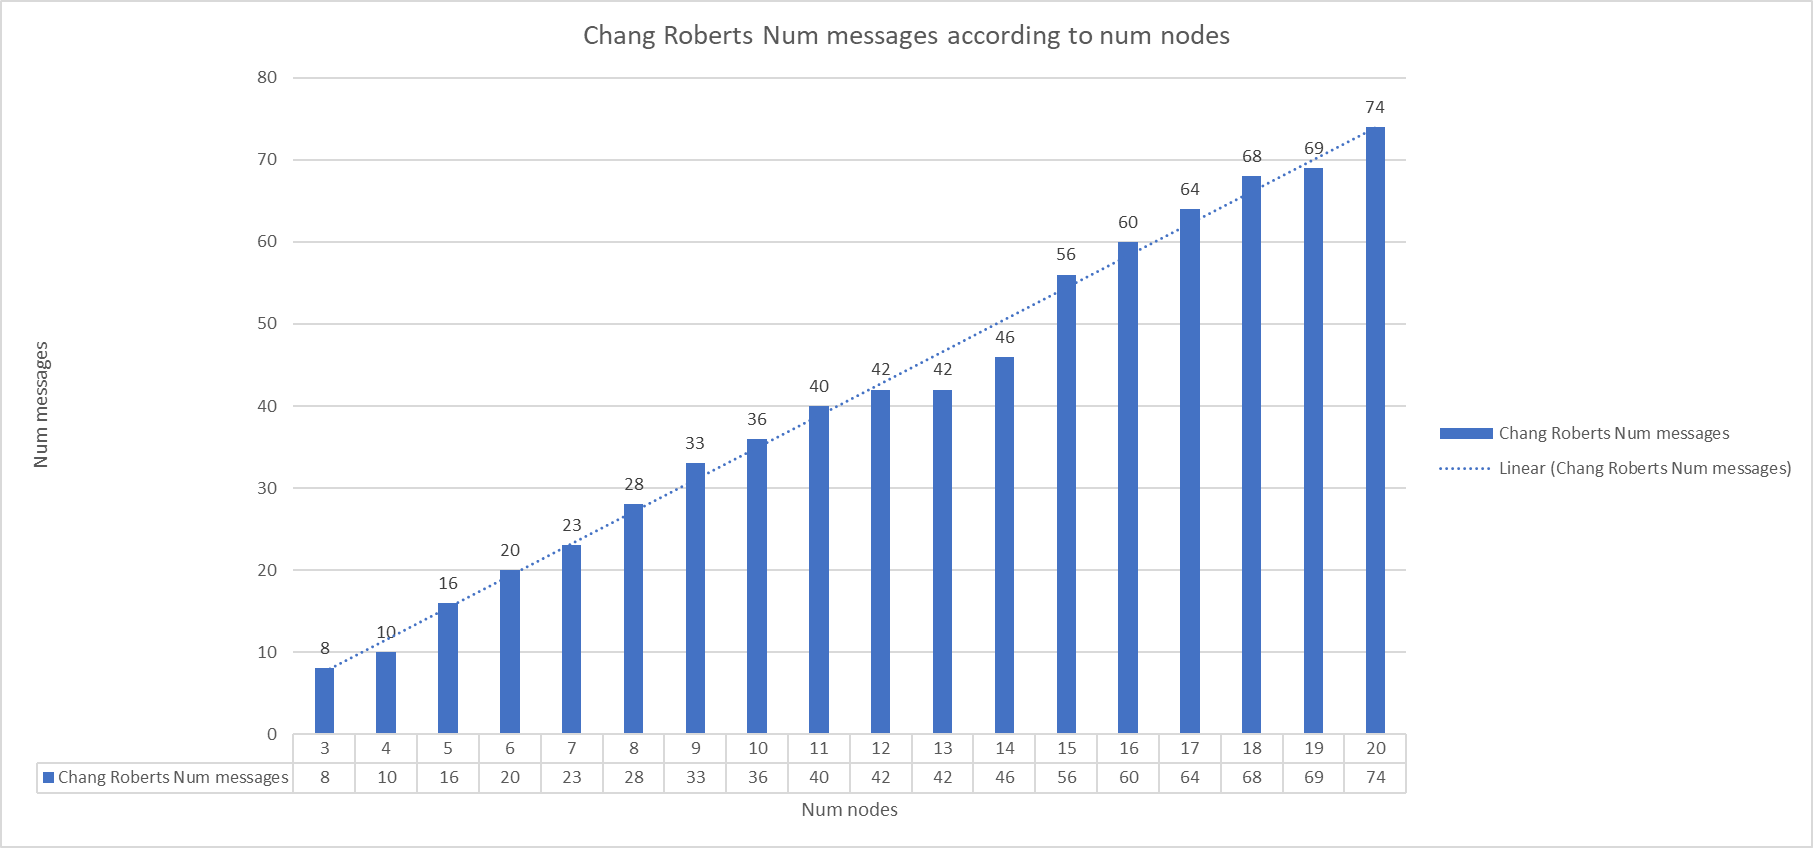
\includegraphics[width=0.8\textwidth]{figures/changroberts_graph.png}
    \caption{Chang Roberts Algorithm}
\end{figure}
\end{frame}

\subsection{franklin's Algorithm}
\begin{frame}
\frametitle{Number of Messages based on Number of Nodes}
\framesubtitle{}

\begin{figure}
    \centering
    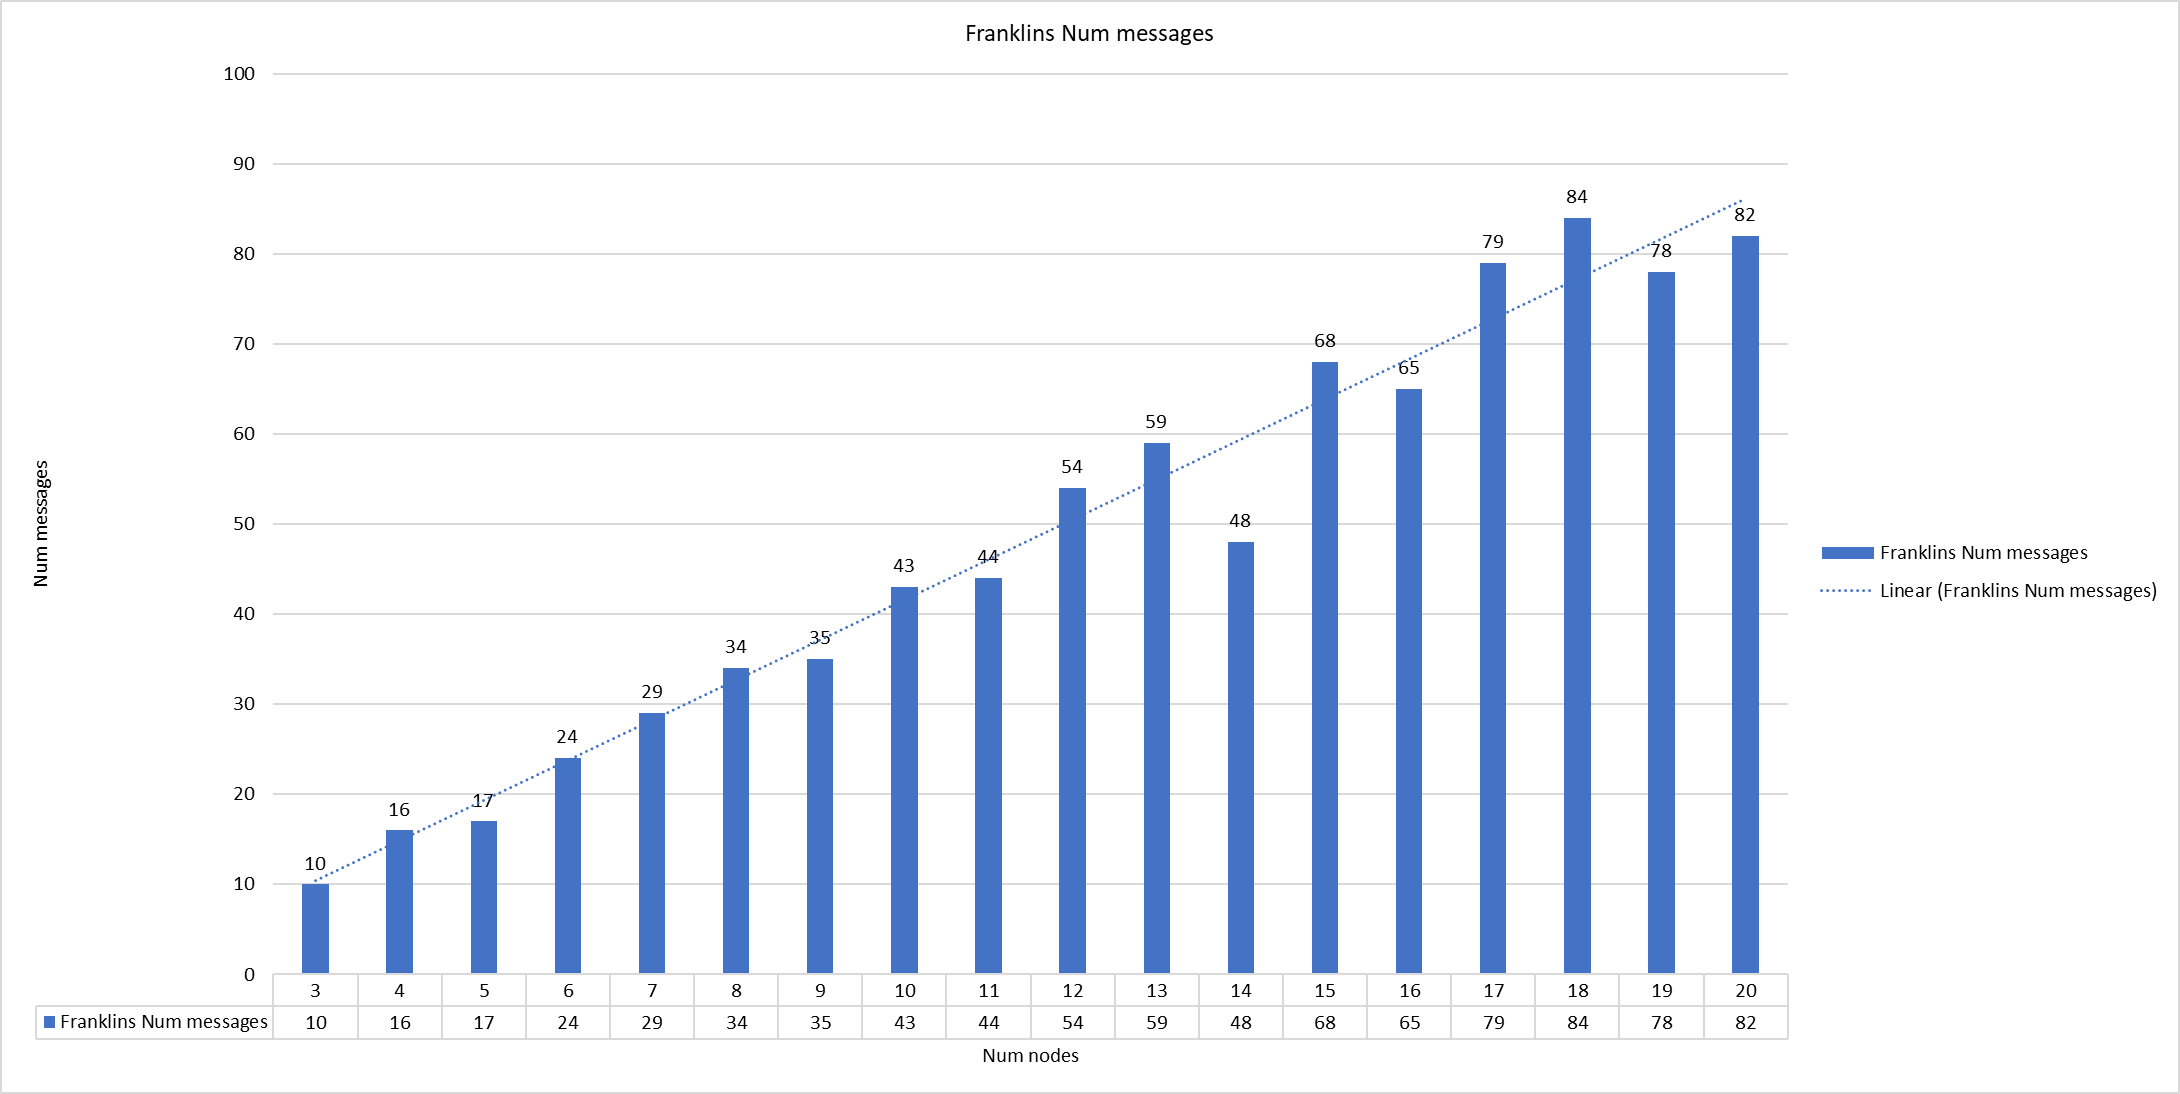
\includegraphics[width=0.8\textwidth]{figures/franklins_graph.png}
    \caption{Franklin's Algorithm}
\end{figure}
\end{frame}

\subsection{Ring Election Algorithms Visualization}
\begin{frame}
\frametitle{How do those algorithms find the leader?}
\framesubtitle{}
Let's proceed with the ring election dance.
\end{frame}

\section{Conclusions}
\begin{frame}
\frametitle{Conclusions}
\framesubtitle{Selecting the Right Leader Election Algorithm for Distributed Systems}
\begin{itemize}
    \item Thorough analysis and comparison of Chang and Roberts Algorithm and Franklin’s Algorithm for leader election in ring networks within distributed systems.
    \item Both algorithms demonstrated effectiveness in leader election, each with its own advantages and disadvantages.
    \item Findings provide insights into selecting appropriate leader election algorithm based on network characteristics and resource constraints.
    \item Future research could explore hybrid approaches or optimizations to address limitations and enhance applicability in diverse distributed system environments.
\end{itemize}

\end{frame}

\section*{References}
\begin{frame}{References}
%\tiny
\bibliographystyle{IEEEtran}
\bibliography{refs}
\nocite{*} % used here because no citation happens in slides
\end{frame}


\thankslide

\end{document}